\documentclass[mathserif]{beamer}

\usepackage{parskip}
\usepackage{amsmath}
\usepackage{amssymb}
\usepackage{graphicx}

\frenchspacing

\logo{
\includegraphics[width=0.075\textwidth]{../Logo}}

\usetheme{Rochester}
\usecolortheme{whale}
%\beamertemplatenavigationsymbolsempty

\AtBeginSection[] {%
	\begin{frame}
		\frametitle{Table of Contents}
		\tableofcontents[currentsection]
	\end{frame}
}

\newenvironment{compactmath}[1][\normalsize]%
	{\begin{minipage}{\textwidth}\vspace{-0.75\baselineskip}#1\begin{equation*}}
	{\end{equation*}\end{minipage}}

\newenvironment{namedframe}[1]%
	{\begin{frame}\frametitle{#1}\framesubtitle{\secname}}
	{\end{frame}}


\usepackage{skull}
\usepackage{tikz}
\usepackage{forest}

\title{Game Theory}
\author{Caroline Liu \and Vincent Macri \and Samantha Unger}
\date{
\includegraphics{../LicenseLogo}\\\copyright{} Caroline Liu, Vincent Macri, and Samantha Unger, 2017}

\newcommand{\emoji}[1]{\raisebox{-0.25\baselineskip}{\includegraphics[height=\baselineskip]{#1}}}

\tikzset{dot/.style= {circle,fill=black,draw,scale=0.5}}

\begin{document}
	\frame{\titlepage}
	\section{Introduction}
	\begin{namedframe}{What is game theory?}
		``Game theory is the study of rigging games in your favour.''
		\sep
		\flushright
		--- Vincent Macri
	\end{namedframe}
	\section{Pick Up Sticks!}
	\sectionstart{The first game}{The most accurately named game of all time.}
	\begin{namedframe}{Rules and intro}
		\alert{Pick up sticks} is a 2 player game that is often used as a game theory question on math contests. The game involves:

		\sep

		Starting with $n$ sticks, the players take turns taking up to $k$ sticks from the total number of sticks until there are none left.

		\sep

		Variations include the winner being the one who takes the last stick, or the loser being the one who takes the last stick.

		\sep

		The game can be structured in such ways that certain players can win every time. Let’s look at some of these scenarios!
	\end{namedframe}
	\begin{namedframe}{The scenarios: your worksheet}
		Let's go over some scenarios.
		\begin{description}[<+(1)->]
			\item[Scenario 1] Whoever picks the last stick \emph{loses}. Which player can guarantee a win?
			\vertspace
			There are 24 sticks in total, and the players can take up to 4 sticks.

			\item[Scenario 2] Whoever picks the last stick \emph{wins}. Which player can guarantee a win?
			\vertspace
			There are 35 sticks, and the players can take up to 4 sticks on their turns.
		\end{description}
	\end{namedframe}
	\bigframe{Try it out yourself!}
	\begin{namedframe}{Answers: The Strats}
		Let's take those scenarios up together.
		\begin{description}[<+(1)->]
			\item[Scenario 1] Player 1 always wins. Why?
			\item[Scenario 2] Player 2 always wins. Why?
		\end{description}
	\end{namedframe}

	\section{Nim}
	\sectionstart{The second game}{Vincent's favourite impartial combinatorial game.}
	\begin{namedframe}{What is an impartial combinatorial game?}
		\begin{itemize}
			\item 2 players
			\item Players alternate turns
			\item Both players can see everything (this rules out most card games)
			\item No chance (this rules out most board games)
			\item Players can make the same moves -- the game is \emph{impartial} (this rules out games such as checkers and chess)
		\end{itemize}
	\end{namedframe}
	\begin{namedframe}{What is Nim?}
		Nim is similar to \emph{pick up sticks}, but with more piles.
		
		\sep

		\begin{itemize}
			\item In Nim, there are $n$ piles, with $k_i$ stones in each pile.
			\item A player can take \emph{as many stones as they want} (as long as they take at least one) from only \emph{one pile} on their turn.
			\item We will be looking at the version where the person who picks up the last stone wins, but Nim can also be played where the person who picks up last loses.
		\end{itemize}

		\sep

		Here is an example Nim game:
		\begin{center}
			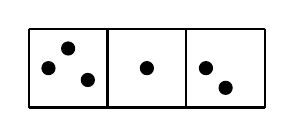
\begin{tikzpicture}
			\draw[step=1cm,black,thick] (0,0) grid(3,1);
				\draw (0.5,0.75) node[dot]{};
				\draw (0.25,0.5) node[dot]{};
				\draw (0.75,0.35) node[dot]{};
				\draw (1.5,0.5) node[dot]{};
				\draw (2.5,0.25) node[dot]{};
				\draw (2.25,0.5) node[dot]{};
			\end{tikzpicture}
		\end{center}
		Here: $n=3$, $k_1 = 3$, $k_2 = 1$, and $k_3 = 2$.
	\end{namedframe}
	\begin{namedframe}{Some Nim notation}
		Instead of drawing out all the boxes with circles in them, we use this notation, because it's shorter and mathematicians are lazy:
		\begin{center}
			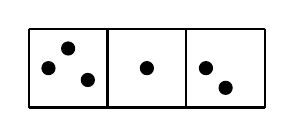
\begin{tikzpicture}
			\draw[step=1cm,black,thick] (0,0) grid(3,1);
				\draw (0.5,0.75) node[dot]{};
				\draw (0.25,0.5) node[dot]{};
				\draw (0.75,0.35) node[dot]{};
				\draw (1.5,0.5) node[dot]{};
				\draw (2.5,0.25) node[dot]{};
				\draw (2.25,0.5) node[dot]{};
			\end{tikzpicture}

			becomes

			$3 \oplus 1 \oplus 2$
		\end{center}
	\end{namedframe}
	\begin{namedframe}{Let's play on the board!}
		\[4 \oplus 5 \oplus 8\]
		\sep
		\[5 \oplus 7\]
		\sep
		\[2 \oplus 2\]
		\sep
		Now, let's look at how to solve Nim.
	\end{namedframe}
	\begin{namedframe}{First, game theory some notation}
		Usually in game theory, we use the following notation:
		\begin{description}
			\item[$N$] The next player wins
			\item[$P$] The previous player wins
		\end{description}
		We write who wins a give game as an ordered pair.

		For example:
		\[(1,N)\]
		\[(1 \oplus 1,P)\]
	\end{namedframe}
	\begin{namedframe}{Game trees}
		\centering
		\only<1>{
			\begin{forest}
				[{$(2 \oplus 2, ?)$}
					[]
					[]
				]
			\end{forest}
		}
		\only<2>{
			\begin{forest}
				[{$(2 \oplus 2, ?)$}
					[{$(1 \oplus 2, ?)$}
						[{$(1 \oplus 1, ?)$}
							[{$(1, ?)$}]
						]
						[{$(2, ?)$}]
						[{$(1, ?)$}]
					]
					[{$(2, ?)$}]
				]
			\end{forest}
		}
		\only<3>{
			\begin{forest}
				[{$(2 \oplus 2, ?)$}
					[{$(1 \oplus 2, ?)$}
						[{$(1 \oplus 1, ?)$}
							[{$(1, N)$}]
						]
						[{$(2, N)$}]
						[{$(1, N)$}]
					]
					[{$(2, N)$}]
				]
			\end{forest}
		}
		\only<4>{
			\begin{forest}
				[{$(2 \oplus 2, P)$}
					[{$(1 \oplus 2, N)$}
						[{$(1 \oplus 1, P)$}
							[{$(1, N)$}]
						]
						[{$(2, N)$}]
						[{$(1, N)$}]
					]
					[{$(2, N)$}]
				]
			\end{forest}
		}
	\end{namedframe}
	\begin{namedframe}{What are the rules for game trees?}
		\begin{itemize}
			\item If the only option is to leave your opponent with an $N$, then it is a $P$.
			\item If you can leave your opponent with a $P$, then it is an $N$.
		\end{itemize}

		\sep

		Game trees are useful, but they take a long time to draw out.

		For example, consider the game tree for:
		\[53 \oplus 242 \oplus 21 \oplus 5 \oplus 13 \oplus 241\]
		It will take a \emph{very} long time to draw this out.

		For some games, including Nim, there is a better way.
	\end{namedframe}
	\begin{namedframe}{Binary}
		First, some quick maths review of base systems and binary.

		In base 10 (decimal) the number $1452$ is really just short for:
		\[1452_{10} = 1 \times 10^3 + 4 \times 10^2 + 5 \times 10^1 + 2 \times 10^0\]

		In base 2 (binary), we only have the digits $0$ and $1$. So:
		\[1001_2 = 1 \times 2^3 + 0 \times 2^2 + 0 \times 2^1 + 1 \times 2^0 = 9_{10}\]
	\end{namedframe}
	\begin{namedframe}{Binary and Nim}
		Take the Nim game $2 \oplus 4 \oplus 7 \oplus 9 \oplus 15$.

		Convert the numbers to binary:
		\[2_{10} = 10_2\]
		\[4_{10} = 100_2\]
		\[7_{10} = 111_2\]
		\[9_{10} = 1001_2\]
		\[15_{10} = 1111_2\]
	\end{namedframe}
	\begin{namedframe}{Sum the binary digits}
		\begin{equation*}
			\begin{array}{ccccccccc}
				2_{10} &\oplus& 4_{10} &\oplus& 3_{10} &\oplus& 9_{10} &\oplus& 15_{10}\\
				10_2   &\oplus& 100_2  &\oplus& 111_2  &\oplus& 1001_2 &\oplus& 1111_2
			\end{array}
		\end{equation*}
		\begin{equation*}
			\begin{array}{rrrr}
				0 & 0 & 1 & 0\\
				0 & 1 & 0 & 0\\
				0 & 1 & 1 & 1\\
				1 & 0 & 0 & 1\\
				1 & 1 & 1 & 1\\\hline
				2 & 3 & 3 & 3
			\end{array}
		\end{equation*}

		\sep

		If any column sum is odd, it is a next player win. If no column sums are odd, it is a previous player win.

		\sep

		How do we apply this?
	\end{namedframe}
	\begin{namedframe}{Applying the general Nim solution}
		Let's go through the following game together on the board, keeping in mind that we want to leave the other player with no odd column sums.
		\sep
		\[2 \oplus 5 \oplus 4\]
	\end{namedframe}
	\begin{namedframe}{Proof of general Nim solution}
		The proof is left as an exercise to the reader, but I'll give two hints:
		\begin{itemize}
			\item It is \emph{not} a coincidence that the $\oplus$ symbol used in Nim is the same symbol used for XOR in boolean algebra.
			\item You can prove it by induction.
		\end{itemize}
		\sep
		If there is time, we can take it up at the end.
	\end{namedframe}

	\section{Chomp!}
	\sectionstart{The third game}{Math has never been this exciting (or delicious) \emoji{Images/ChocolateBarEmoji}}
	\begin{namedframe}{What's the game?}
		Chomp is played on a rectangular grid, such as squares of a candy bar.
		The lower left square is considered \alert{poison}.
		Players take turns picking a square.
		With each choice, all squares above and to the right of the picked square are no longer available -- they are eaten.
		The person forced to take the \alert{poison} square loses.
		\begin{center}
			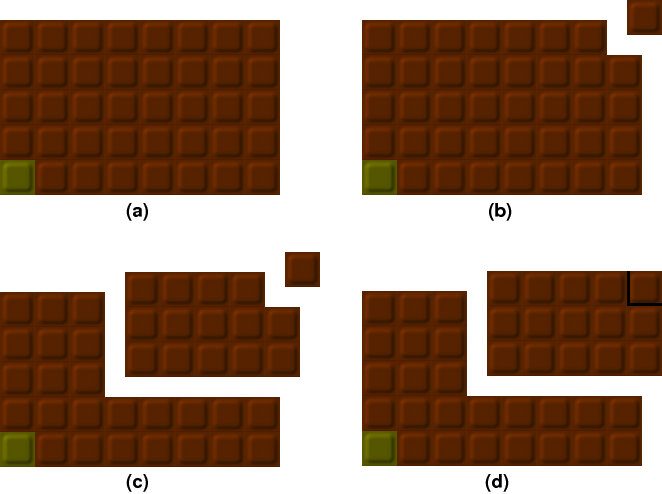
\includegraphics[width=0.6\textwidth]{Images/Chomp1}
		\end{center}
	\end{namedframe}
	\begin{namedframe}{Let's play! ($4 \times 6$ board)}
		\begin{center}
			\begin{tikzpicture}
				\draw[step=1.5cm,black,thick] (0,0) grid(6 * 1.5,4 * 1.5);
				\draw (0.75,0.75) node {\Huge\emoji{Images/SkullEmoji}};
			\end{tikzpicture}
		\end{center}
	\end{namedframe}
	\begin{namedframe}{Is there a winning strategy? (Or, why this game so cool.)}
		Yes!
		\begin{itemize}[<+(1)->]
			\item The first player has a winning strategy for any finite grid.
				\begin{itemize}
					\item They can take any move that the second can player can make, that would result in winning.
					\begin{itemize}
						\item We can think of this as strategy stealing!
					\end{itemize}
				\end{itemize}
		\end{itemize}
		\pause
		The real question is\ldots
	\end{namedframe}
	\begin{namedframe}{What is the winning strategy?}
		\begin{itemize}[<+->]
			\item Does anyone know one right away?
			\item No!
			\item Let's analyze some cases!
		\end{itemize}
	\end{namedframe}
	\begin{namedframe}{$n \times n$ grid}
		\begin{itemize}[<+->]
			\item What's the strategy here?
			\item Make an ``L'', and then take symmetrical moves!
		\end{itemize}
		\begin{center}
			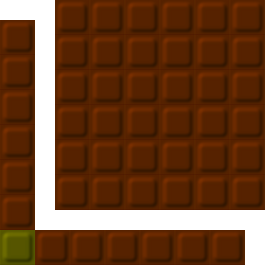
\includegraphics[width=0.5\textwidth]{Images/Chomp2}
		\end{center}
	\end{namedframe}
	\begin{namedframe}{$2 \times n$ grid}
		\begin{itemize}[<+->]
			\item What's the strategy here?
			\item Make sure that player 2 encounters a rectangle\ldots{} with a square missing!
		\end{itemize}
		\begin{center}
			
\includegraphics[width=\textwidth]{Images/Chomp3}
		\end{center}
	\end{namedframe}
	\begin{namedframe}{What is the winning strategy?}
		\begin{itemize}[<+(1)->]
			\item Just because there is always a winning strategy for player 1 doesn't mean that we know what it is!
			\item We know the strategy for $n \times n$ and $2 \times n$, as well as particular small grids\ldots{} but not all\ldots
			\begin{itemize}
				\item In 2002, Steven Byrnes (a high school senior!!) solved the $3 \times n$ case and won over $\$100\,000$
				\item Computers can calculate winning moves for grids of reasonable size
			\end{itemize}
		\end{itemize}
	\end{namedframe}
	\begin{namedframe}{Some cool extensions}
		\begin{columns}
			\begin{column}{0.5\textwidth}
				\begin{itemize}
					\item $3$D or $n$D chomp
					\item Infinite/ordinal chomp:
					\begin{itemize}
						\item Here is how player ``Too'' can win on a $2 \times \omega$ board
					\end{itemize}
				\end{itemize}
			\end{column}
			\begin{column}{0.5\textwidth}
				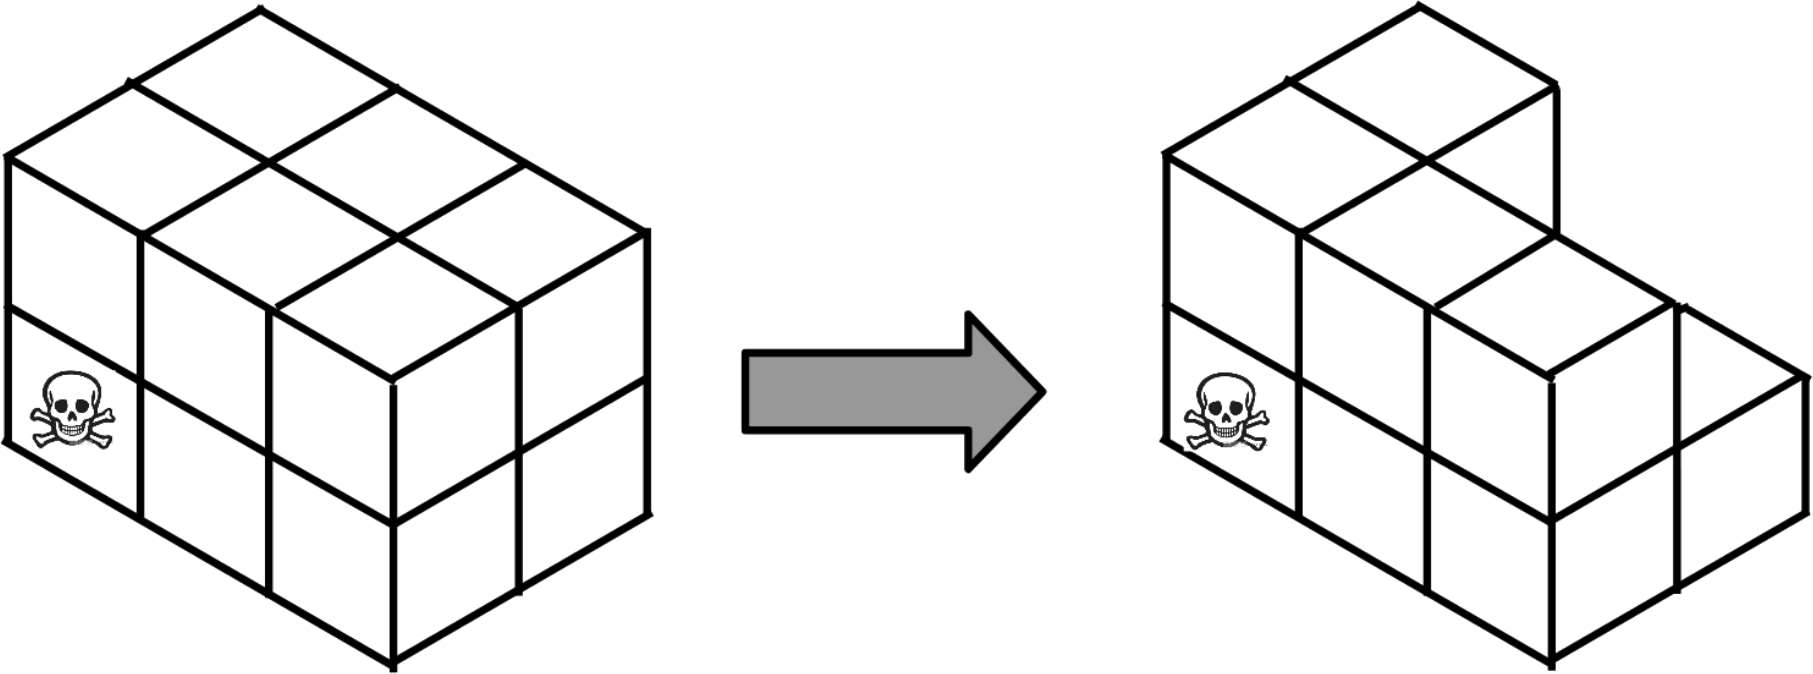
\includegraphics[width=\textwidth]{Images/Chomp3D}
			\end{column}
		\end{columns}
		\begin{center}
			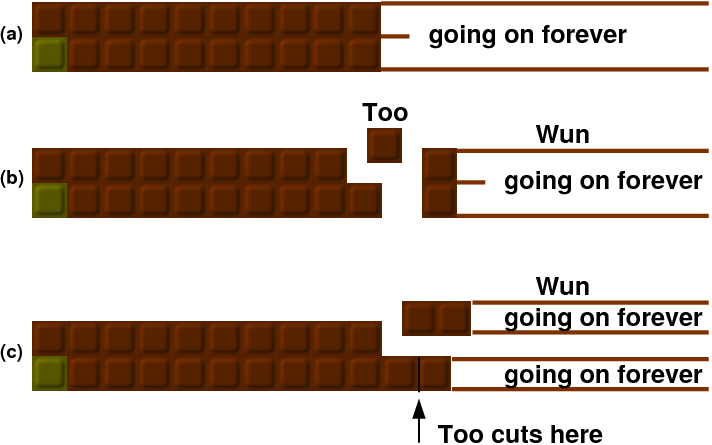
\includegraphics[width=0.75\textwidth]{Images/Chomp4}
		\end{center}
	\end{namedframe}

\end{document}
